157. \begin{figure}[ht!]
\center{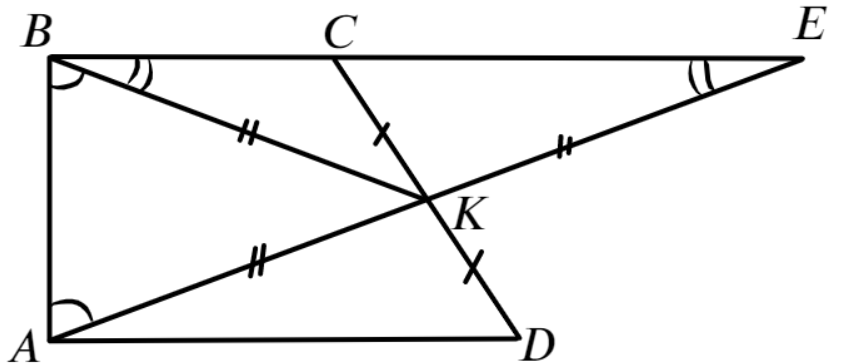
\includegraphics[scale=0.35]{g8-157.png}}
\end{figure}\\
Продлим $AK$ до пересечения с продолжением $BC$ в точке $E.$  В треугольниках $ADK$ и $KCE:\ DK=KC,\ \angle AKD=\angle CKE\ (\text{вертикальные})$ и $\angle ADK=\angle KCE$ (накрест лежащие), значит эти треугольники равны по второму признаку и $AK=KE.$ Так как $\angle BAK=\angle ABK,$ треугольник $ABK$ является равнобедренным и $AK=BK,$ поэтому $KE=BK=AK$ и треугольник $BKE$ также является равнобедренным и  $\angle KBE=\angle KEB.$ Пусть $\angle KBE=x,$ а $\angle BAK=y,$ тогда запишем сумму углов треугольника $ABE:\ 2x+2y=180^\circ,\ x+y=90^\circ.$ Значит, $\angle BAD=90^\circ.$\\
